\chapter{Two more tests of CSC-LISTA}\label{ch:followups}

Chapter~\ref{ch:results} left two open questions about strict Eq.~20 at 64 layers. Its simulated validation error was
best very early (step 200 of 1,000) and then got worse. Was it overfitting the 200 stored layouts? And does training on
MSE, when we score relative $L_2$, hold it back? On 6 November we ran one test for each. Both kept everything else
strict: same dictionary, same 64 layers, same 1,000 steps of 8 crops of 512 pixels.

\section{Test 1: a new layout for every crop}

The trainer gained a \code{--stream} option. Instead of cutting crops from the 200 stored layouts, it simulates a brand-new
current layout for every crop. Over 1,000 steps of 8 crops that is 8,000 layouts, so the network never sees the same wires
twice. If the early peak were overfitting, it should disappear.

\section{Test 2: the relative loss, and nothing else}

The second test switched only the loss to per-crop relative $L_2$, the same quantity we score. This is \textbf{our
addition}, not part of Eq.~20. The earlier relative runs in Chapter~\ref{ch:density} also had the threshold floor, so this
was the first clean test of the loss alone. It ran on the stored layouts and again with streaming.

\section{Results}

\begin{center}
\begin{tabular}{lcc}
\toprule
Strict Eq.~20, 64 layers & Simulated validation & COMSOL (15 pairs) \\
\midrule
MSE, 200 stored layouts (Chapter~\ref{ch:results}) & 48.8\% & \textbf{33.8\%} \\
MSE, 8,000 streamed layouts & 49.3\% & 36.0\% \\
Relative loss, 200 stored layouts & 41.0\% & 35.6\% \\
Relative loss, 8,000 streamed layouts & \textbf{40.9\%} & 36.2\% \\
\bottomrule
\end{tabular}
\end{center}

\begin{figure}[H]
\centering
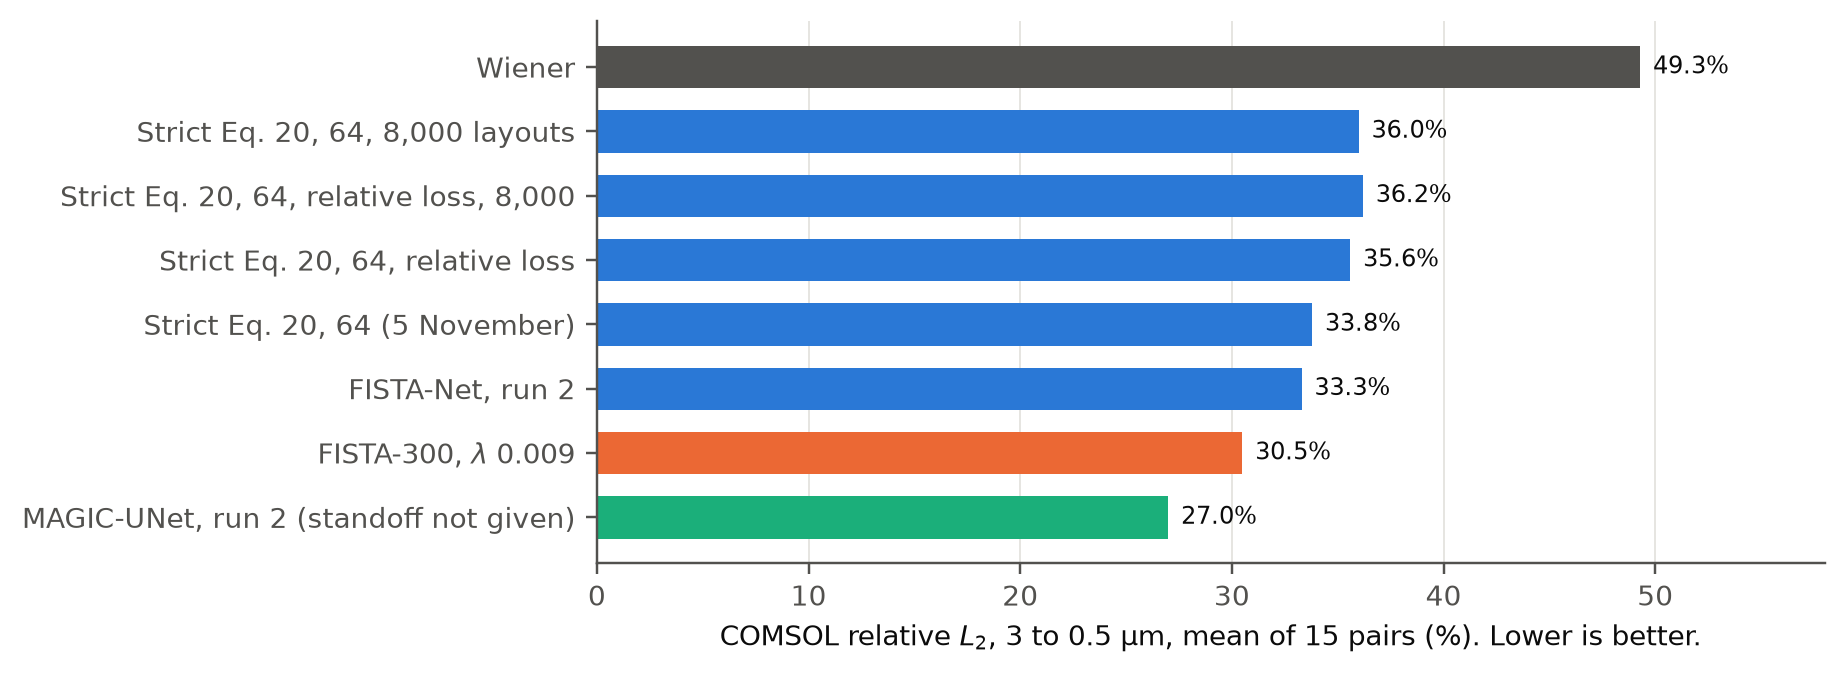
\includegraphics[width=\textwidth]{results_now}
\caption{COMSOL scores at 3\um\ to 0.5\um\ after 5 November, with the earlier best results for comparison. Blue bars are
CSC-LISTA and FISTA-Net, orange is FISTA, green is MAGIC-UNet (Chapters~\ref{ch:magic} and~\ref{ch:magic_results}).}
\label{fig:results_now}
\end{figure}

\begin{keyidea}[What the two tests mean]
\begin{itemize}
\item \textbf{More data did not help.} With 8,000 layouts the validation error still peaked early (step 100) and then
rose. So the early peak is not overfitting. It is a mismatch between the training loss and the score.
\item \textbf{The relative loss fixed that mismatch on simulation:} validation fell from 48.8\% to 41.0\%. But COMSOL got
\emph{worse}, 35.6\% against 33.8\%.
\item So the limit is neither data volume nor the loss. It is the gap between our simulator and COMSOL. Making the network
better at simulated data made it slightly worse at COMSOL.
\end{itemize}
\end{keyidea}

\begin{careful}
Each run used one seed, and the COMSOL differences are about 2 points. That is enough to say these changes did not help,
but not enough to rank the four runs against each other.
\end{careful}

\begin{defend}[If your professor asks: did you try more training data?]
Yes. A fresh simulated layout for every crop, 8,000 in all, gave 36.0\% on COMSOL against 33.8\% with 200 layouts. Data
volume is not what limits CSC-LISTA.
\end{defend}
